\documentclass{article}

\usepackage{amsmath, amsthm, amssymb, amsfonts}
\usepackage{thmtools}
\usepackage{graphicx}
\usepackage{stmaryrd}

\newtheorem{theorem}{Theorem}

\begin{document}

\begin{figure}
    \centering
    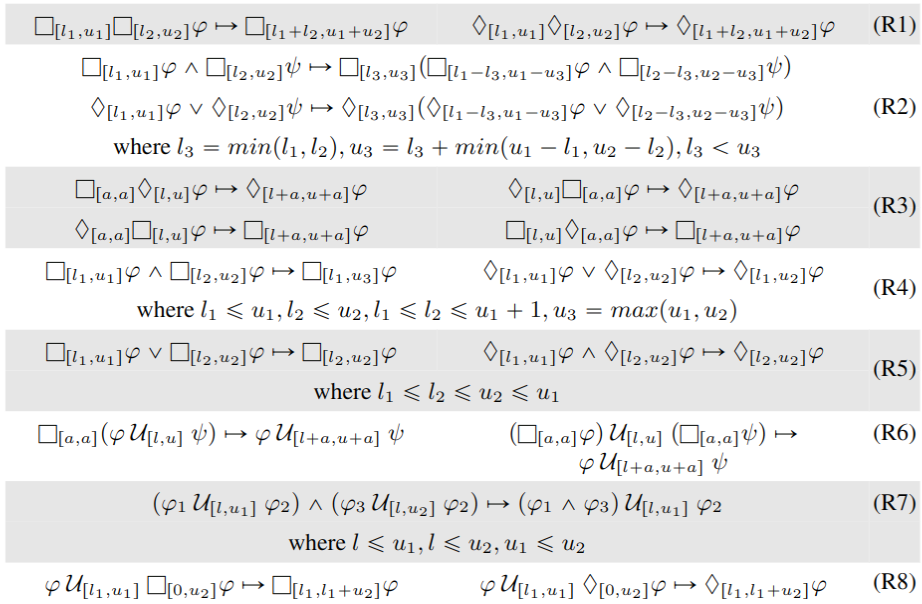
\includegraphics[width=0.9\textwidth]{rewrite_rules.png} 
    \hfill \\
    \bf Figure 2
\end{figure}

\begin{theorem}{\emph{\bf(Equivalence of MLTL Rewrite Rules)}}
Let $\varphi, \psi, \varphi_1, \varphi_2, \varphi_3$ be well-formed MLTL formulas and $a$, $l$, $u$, $l_1$, $u_2$, $l_2$, $u_2$, $l_3$, $u_3 \in \mathbb{N}_0$ such that $l \leq u$, $l_1 \leq u_1$, $l_2 \leq u_2$, $l_3 \leq u_3$. Then each rewrite relation ($\mapsto$) in Fig 2 is also an equivalence relation.
\end{theorem}

\begin{proof}
We prove each rule in Figure 2 is semantics-preserving i.e., the right- and left-hand sides of the $\mapsto$ operator are equivalent. Recall that two MLTL formulas $\varphi,\psi$ are equivalent only if $\pi \models \varphi \leftrightarrow \pi \models \psi$ for all $\pi$.

\begin{enumerate}
    \item[(R1)] Let $\varphi$ be an MLTL formula, $\pi$ be a trace, and $l_1 \leq u_1, l_2 \leq u_2$. We prove
    $$
        \pi \models \Box_{[l_1,u_1]}{\Box_{[l_2,u_2]}{\varphi}} \leftrightarrow \pi \models \Box_{[l_1+l_2,u_1+u_2]}{\varphi}.
    $$
    
    \begin{enumerate}
        \item[($\rightarrow$)] Let $\pi$ be defined such that $\pi \models \Box_{[l_1,u_1]}{\Box_{[l_2,u_2]}{\varphi}}$. We show that $\pi \models \Box_{[l_1+l_2,u_1+u_2]}{\varphi}$ using the MLTL semantics. 
        By the semantics of $\Box_{I}{}$, we know that for each $i \in [l_1,u_1]$, $\pi_i \models \Box_{[l_2,u_2]}{\varphi}$. 
        Intuitively, this means that $\pi$ satisfies $\varphi$ at timestamps $[l_2,u_2]$ relative to $i$ i.e., $\pi \models \varphi$ starting at timestamp $i+l_2$ and ending at timestamp $i+u_2$.
        So, applying the semantics of $\Box_{I}{}$ again, we have that $\pi_{i+j} \models \varphi$ for each $i \in [l_1,u_1]$, $j \in [l_2,u_2]$.  
        By the definition of trace suffixes, this means that $\pi_k \models \varphi$ for each $k \in [l_1+l_2,u_1+u_2]$.
        Therefore $\pi \models \Box_{[l_1+l_2,u_1+u_2]}{\varphi}$.
        \item[($\leftarrow$)] Let $\pi$ be defined such that $\pi \models \Box_{[l_1+l_2,u_1+u_2]}{\varphi}$. 
        We show that  $\pi \models \Box_{[l_1,u_1]}{\Box_{[l_2,u_2]}{\varphi}}$.
        Then $\pi_k \models \varphi$ for all $k \in [l_1+l_2,u_1+u_2]$. 
        Splitting this interval into two intervals, we have that $\pi_{i+j} \models \varphi$ for each $i \in [l_1,u_1]$, $j \in [l_2,u_2]$, as in the converse proof. 
        Then $\pi \models \Box_{[l_1,u_1]}{\Box_{[l_2,u_2]}{\varphi}}$ by the semantics of $\Box_{I}$.
    \end{enumerate}
    The proof for the $\lozenge$ version of (R1) is symmetric.


    \item[(R2):] Let $\varphi,\psi$ be MLTL formulas and $l_1 \leq u_1, l_2 \leq u_2$. We prove 
    $$
        \Box_{[l_1,u_1]}{\varphi} \lor \Box_{[l_2,u_2]}{\psi} \equiv \Box_{[l_3,u_3]}{(\Box_{[l_1-l_3,u_1-u_3]}{\varphi} \lor \Box_{[l_2-l_3,u_2-u_3]}{\psi})}
    $$ 
    for any $l_3 = min(l_1,l_2)$, $u_3 = l_3 + min(u_1-l_1,u_2-l_2)$, $l_3 < u_3$ using established equivalences and the MLTL semantics. 
    Using (R1), we see that 
    $$
        \Box_{[l_1,u_1]}{\varphi} \land \Box_{[l_2,u_2]}{\psi} \equiv \Box_{[l_3,l_3]}{\Box_{[l_1-l_3,u_1-l_3]}{\varphi} \land \Box_{[l_3,l_3]}{\Box_{[l_2-l_3,u_2-l_3]}{\psi}}}.
    $$
    This follows if both intervals $[l_1-l_3,u_1-l_3]$, $[l_2-l_3,u_2-l_3]$ are valid i.e., (a) $l_1-l_3 \geq 0$, (b) $l_2-l_3 \geq 0$, and (c) $l_1-l_3 \leq u_1-l_3$, (d) $l_2-l_3 \leq u_2-l_3$. 
    \begin{enumerate}
    \item Recall that $l_3 = l_1$, then $l_3 \leq l_1$.
    \item Recall that $l_3 = l_1 \leq l_2$, then $l_2-l_3 \geq 0 \rightarrow l_2 \geq l_3 \rightarrow l_3 \leq l_2$ holds.
    \item Since $l_1 \leq u_1$, we see that $l_1-l_3 \leq u_1-l_3 \rightarrow l_1 \leq u_1$ holds.
    \item Since $l_2 \leq u_2$, we see that $l_2-l_3 \leq u_2-l_3 \rightarrow l_2 \leq u_2$ holds.
    \end{enumerate}
Now, let $u_3 = l_3+min(u_1-l_1,u_2-l_2)$. Applying (R1) once more, we have
\begin{align*}
& \Box_{[l_3,l_3]}{\Box_{[l_1-l_3,u_1-l_3]}{\varphi} \land \Box_{[l_3,l_3]}{\Box_{[l_2-l_3,u_2-l_3]}{\psi}}} \equiv \\ 
& \qquad \qquad \Box_{[l_3,u_3]}{\Box_{[l_1-l_3,u_1-u_3]}{\varphi}} \land \Box_{[l_3,u_3]}{\Box_{[l_2-l_3,u_2-u_3]}{\psi}}
\end{align*}
Since this only affects the upper bounds of the inner $\Box_{}{}$ operators, we show that (a) $l_1-l_3 \leq u_1-u_3$ and (b) $l_2-l_3 \leq u_2-u_3$.
    \begin{enumerate}
    \item Consider the two cases of $u_1-l_1 \leq u_2-l_2$ and $u_2-l_2 < u_1-l_1$:
        \begin{enumerate}
            \item Assume $u_1-l_1 \leq u_2-l_2$, then $u_3 = u_1-l_1+l_3$. 
                Replacing this in the target inequality, we have 
                $$
                    l_1-l_3 \leq u_1-(u_1-l_1+l_3) \rightarrow l_1-l_3 \leq l_1-l_3.
                $$
            \item Otherwise, $u_2-l_2 < u_1-l_1$. 
                Then $u_3 = u_2-l_2+l_3$, and replacing this in the target inequality, we have 
                $$
                    l_1-l_3 \leq u_1-(u_2-l_2+l_3) \rightarrow 0 \leq u_1-l_3-(u_2-l_2) \rightarrow u_2-l_2 \leq u_1-l_3.
                $$ 
                Now, since $l_3=l_1$, we have $u_2-l_2 \leq u_1-l_1$ which is true from our assumption. 
                \end{enumerate}
    
    \item 
        Consider the two cases of $u_1-l_1 \leq u_2-l_2$ and $u_2-l_2 < u_1-l_1$:
        \begin{enumerate}
            \item Assume $u_1-l_1 \leq u_2-l_2$, then $u_3 = u_1-l_1+l_3$. 
                Replacing this in the target inequality, we have 
                \begin{align*}
                    & l_2-l_3 \leq u_2-(u_1-l_1+l_3) \rightarrow l_2-l_3 \leq u_2-u_1+l_1-l_3 \rightarrow \\
                    & \qquad l_2 \leq u_2-u_1+l_1 \rightarrow u_1-l_1 \leq u_2-l_2,
                \end{align*}
                which is true from our assumption.
            \item Otherwise, $u_2-l_2 < u_1-l_1$, then $u_3 = u_2-l_2+l_3$.
                Replacing this in the target inequality, we have 
                \begin{align*}
                    & l_2-l_3 \leq u_2-(u_2-l_2+l_3) \rightarrow l_2-l_3 \leq u_2-u_2+l_2-l_3 \rightarrow \\
                    & \qquad l_2 \leq u_2-u_2+l_2 \rightarrow l_2 \leq l_2.
                \end{align*} 
            \end{enumerate}
    
    \end{enumerate}
Finally, let $\pi$ be a trace. We prove that
\begin{align*}
    &  \pi \models \Box_{[l_3,u_3]}{\Box_{[l_1-l_3,u_1-l_3-u_3]}{\varphi}} \land \Box_{[l_3,u_3]}{\Box_{[l_2-l_3,u_2-l_3-u_3]}{\psi}} \leftrightarrow \\ 
    & \qquad \qquad \pi \models \Box_{[l_3,u_3]}{(\Box_{[l_1-l_3,u_1-l_3-u_3]}{\varphi} \land \Box_{[l_2-l_3,u_2-l_3-u_3]}{\psi})}.
\end{align*} 
    \begin{enumerate}
    \item  ($\rightarrow$)
        Let $\pi$ be defined such that $\pi \models (\Box_{[l_3,u_3]}{\Box_{[l_1,u_1]}{\varphi}}) \land (\Box_{[l_3,u_3]}{\Box_{[l_2,u_2]}{\psi}})$.
        We show that $\pi \models \Box_{[l_3,u_3]}{(\Box_{[l_1-l_3,u_1-l_3-u_3]}{\varphi} \land \Box_{[l_2-l_3,u_2-l_3-u_3]}{\psi})}$ using the MLTL semantics.
        We apply the semantic definitions of $\land$ and $\Box_{I}{}$ to see that $\pi_i \models \Box_{[l_1,u_1]}{\varphi}$ and $\pi_i \models \Box_{[l_2,u_2]}{\psi}$ for all $i \in [l_3,u_3]$. 
        Combining these relations using the semantics of $\land$ once more, we see that $\pi_i \models \Box_{[l_1,u_1]}{\varphi} \land \Box_{[l_2,u_2]}{\psi}$ for all $i \in [l_3,u_3]$.
        Using the semantics of $\Box_{I}{}$ again, we see that $\pi \models \Box_{[l_3,u_3]}{(\Box_{[l_1,u_1]}{\varphi} \land \Box_{[l_2,u_2]}{\psi})}$.
    
    \item  ($\leftarrow$)
        Conversely, let $\pi$ be defined such that $\pi \models \Box_{[l_3,u_3]}{(\Box_{[l_1,u_1]}{\varphi} \land \Box_{[l_2,u_2]}{\psi})}$.
        We show that $\pi \models (\Box_{[l_3,u_3]}{\Box_{[l_1,u_1]}{\varphi}}) \land (\Box_{[l_3,u_3]}{\Box_{[l_2,u_2]}{\psi}})$ using the MLTL semantics.
        Then $\pi_i \models \Box_{[l_1,u_1]}{\varphi}$ and $\pi_i \models \Box_{[l_2,u_2]}{\psi}$ for all $i \in [l_3,u_3]$.
        Using the semantic definitions of $\land$ and $\Box_{I}{}$, we see that $\pi \models \Box_{[l_3,u_3]}{\Box_{[l_1,u_1]}{\varphi}}$ and $\pi \models \Box_{[l_3,u_3]}{\Box_{[l_2,u_2]}{\psi}}$, so $\pi \models (\Box_{[l_3,u_3]}{\Box_{[l_1,u_1]}{\varphi}}) \land (\Box_{[l_3,u_3]}{\Box_{[l_2,u_2]}{\psi}})$.
    
    \end{enumerate}

The proof for the $\lozenge$ version of (R2) is symmetric.



    \item[(R3):] Let $\varphi$ be a MLTL formula and $l \leq u$. 
We prove 
$$
    \Box_{[a,a]}{\lozenge_{[l,u]}{\varphi}} \equiv \lozenge_{[l,u]}{\Box_{[a,a]}{\varphi}}
$$
using established MLTL equivalences.
Using Equation 3 and (R1) to expand the expression until we have $a$ of the $\Box_{[1,1]}{}$ operators in lines 3 and 9 of the following proof we can show:
\begin{align*}
    \Box_{[a,a]}{\lozenge_{[l,u]}{\varphi}} & \equiv \Box_{[1,1]}{\Box_{[a-1,a-1]}{\lozenge_{[l,u]}{\varphi}}} \\
    & \equiv \cdots \text{Applying } a \text{ times} \\
    & \equiv \Box_{[1,1]}{\cdots \Box_{[1,1]}{\lozenge_{[l,u]}{\varphi}}} \\
    & \equiv \lozenge_{[1,1]}{\cdots \lozenge_{[1,1]}{\lozenge_{[l,u]}{\varphi}}} \\
    & \equiv \lozenge_{[l+a,u+a]}{\varphi} \\
    & \equiv \lozenge_{[l+a-1,u+a-1]}{\lozenge_{[1,1]}{\varphi}} \\
    & \equiv \cdots \text{Applying } a \text{ times} \\
    & \equiv \lozenge_{[l,u]}{\lozenge_{[1,1]}{\cdots \lozenge_{[1,1]}{\varphi}}} \\
    & \equiv \lozenge_{[l,u]}{\Box_{[1,1]}{\cdots \Box_{[1,1]}{\varphi}}} \\
    & \equiv \lozenge_{[l,u]}{\Box_{[a,a]}{\varphi}}.
\end{align*} 
The proof for the $\lozenge_{[a,a]}$ version of (R3) is symmetric.



    \item[(R4):] Let $\varphi$ be a MLTL formula and $l_1 \leq u_1$, $l_2 \leq u_2$, $l_1 \leq l_2 \leq u_1 + 1$, $u_3 = max(u_1, u_2)$. We prove that 
$$
    \Box_{[l_1,u_1]}{\varphi} \land \Box_{[l_2,u_2]}{\varphi} \equiv \Box_{[l_1,u_3]}{\varphi}.
$$
We first show that $ \pi \models \Box_{[l,l]}{\varphi} \land \Box_{[l+1,u]}{\varphi} \leftrightarrow \pi \models  \Box_{[l,u]}{\varphi}$ for any trace $pi$ and $l < u$. 
    \begin{enumerate}
    \item  $(\rightarrow)$
        Let $\pi$ be a trace such that $\pi \models \Box_{[l,l]}{\varphi} \land \Box_{[l+1,u]}{\varphi}$. 
        We show that $\pi \models \Box_{[l,u]}{\varphi}$. 
        From the semantics of $\Box_{}{}$ and (R1), we see that $\pi_i \models \varphi$ for all $i \in [l,l]$ and $\pi_j \models \varphi$ for all $j \in [l+1,u]$. 
        Now, since $[l,l] \cup [l+1,u] = [l,u]$, it follows that $\pi_k \models \varphi$ for all $k \in [l,u]$.
        This matches the semantic definition of $\Box_{}{}$ and therefore $\pi \models \Box_{[l,u]}{\varphi}$.
     
    \item  $(\leftarrow)$
        Conversely, if $\pi$ is a trace such that $\pi \models \Box_{[l,u]}{\varphi}$, then $\pi \models \Box_{[l,l]}{\varphi} \land \Box_{[l+1,u]}{\varphi}$ because $\pi_i \models \varphi$ for all $i \in [l,u]$ where $[l,l] \cup [l+1,u] = [l,u]$ as before.
    
    \end{enumerate}
From above, we can expand each $\Box_{I}{}$ operator to a conjunction of singleton intervals, remove repeated conjunctive clauses, then use the above equivalence again to simplify:
\begin{align*}
    \Box_{[l_1,u_1]}{\varphi} \land \Box_{[l_2,u_2]}{\varphi} \equiv & (\Box_{[l_1,l_1]}{\varphi} \land \Box_{[l_1+1,u_1]}) \land \Box_{[l_2,u_2]}{\varphi} \\
    \equiv & \cdots \text{Applying } u_1-l_1 \text{ times}  \\
    \equiv & (\Box_{[l_1,l_1]}{\varphi} \land \cdots \land \Box_{[u_1,u_1]}{\varphi}) \land \Box_{[l_2,u_2]}{\varphi} \\
    \equiv & (\Box_{[l_1,l_1]}{\varphi} \land \cdots \land \Box_{[u_1,u_1]}{\varphi}) \land (\Box_{[l_2,l_2]}{\varphi} \land \Box_{[l_2+1,u_2]}{\varphi}) \\
    \equiv & \cdots \text{Applying } u_2-l_2 \text{ times}  \\
    \equiv & \Box_{[l_1,l_1]}{\varphi} \land \cdots \land \Box_{[u_1,u_1]}{\varphi} \land (\Box_{[l_2,l_2]}{\varphi} \land \cdots \land \Box_{[u_2,u_2]}{\varphi}) \\
    \equiv & \Box_{[l_1,l_1]}{\varphi} \land \cdots \land \Box_{[l_2-1,l_2-1]}{\varphi} \land \Box_{[l_2,l_2]}{\varphi} \land \cdots \land \Box_{[u_2,u_2]}{\varphi} \\
    \equiv & \Box_{[l_1,l_1+1]}{\varphi} \land \cdots \land \Box_{[l_2-1,l_2-1]}{\varphi} \land \Box_{[l_2,l_2]}{\varphi} \land \cdots \land \Box_{[u_2,u_2]}{\varphi} \\
    \equiv & \cdots \text{Applying } l_2-l_1-1 \text{ times} \\
    \equiv & \Box_{[l_1,l_2-1]}{\varphi} \land \Box_{[l_2,l_2]}{\varphi} \land \cdots \land \Box_{[u_2,u_2]}{\varphi} \\
    \equiv & \cdots \text{Applying } u_2-l_2+1 \text{ times}  \\
    \equiv & \Box_{[l_1,u_2]}{\varphi} 
\end{align*}
Note that from lines 6 to 7 we remove repeated clauses e.g., $l_2 \leq u_1 \leq u_2$ so there must be two instances of the expression $\Box_{[u_1,u_1]}{\varphi}$ in the formula.

The proof for the $\lozenge$ version of (R4) is symmetric.


    \item[(R5):] Let $\varphi$ be a MLTL formula and $l_1 \leq l_2 \leq u_2 \leq u_1$. We prove that 
$$
\Box_{[l_1,u_1]}{\varphi} \lor \Box_{[l_2,u_2]}{\varphi} \equiv \Box_{[l_2,u_2]}{\varphi}.
$$

We first show that 
$$
    \pi \models \Box_{[l,u_1]}{\varphi} \lor \Box_{[l,u_2]}{\varphi} \leftrightarrow \pi \models \Box_{[l,u_1]}{\varphi}
$$ 
for any trace $\pi$.
    \begin{enumerate}
    \item  $(\rightarrow)$
        Assume for the purposes of contraction that $\pi$ is a trace such that $\pi \models \Box_{[l,u_1]}{\varphi} \lor \Box_{[l,u_2]}{\varphi}$ but $\pi \nvDash \Box_{[l,u_1]}{\varphi}$. 
        Therefore there is some $i \in [l,u_1]$ such that $\pi_i \nvDash \varphi$. 
        By (R1), we see that
        $$
        \Box_{[l,u_1]}{\varphi} \lor \Box_{[l,u_2]}{\varphi} \equiv \Box_{[l,u_1]}{\varphi} \lor \Box_{[0,u_2-u_1]}{\Box_{[l,u_1]}{\varphi}}
        $$
        But $\pi \nvDash \Box_{[l,u_1]}{\varphi} \lor \Box_{0,u_2-u_1}{\Box_{[l,u_1]}{\varphi}}$ since $\pi \nvDash \Box_{[l,u_1]}{\varphi}$. 
        Therefore if $\pi \models \Box_{[l,u_1]}{\varphi} \lor \Box_{[l,u_2]}{\varphi}$, then $\pi \models \Box_{[l,u_1]}{\varphi}$.
    
    \item  $(\leftarrow)$
        Conversely, assume that $\pi$ is a trace such that $\pi \models \Box_{[l,u_1]}{\varphi}$ but $\pi \nvDash \Box_{[l,u_1]}{\varphi} \lor \Box_{[l,u_2]}{\varphi}$. 
        But this is a contradiction, since by the definition of disjunction, if $\pi \models \Box_{[l,u_1]}{\varphi}$, then $\pi \models \Box_{[l,u_1]}{\varphi} \lor \Box_{[l,u_2]}{\varphi}$ since the left-hand disjunctive clause models $\pi$.
        Therefore if $\pi \models \Box_{[l,u_1]}{\varphi}$, then $\pi \models \Box_{[l,u_1]}{\varphi} \lor \Box_{[l,u_2]}{\varphi}$.
    
    \end{enumerate}
Next we consider the cases for when $l_1 < l_2$ and $l_1 = l_2$.
    \begin{enumerate}
    \item  $(l_1 < l_2)$
        Starting from the left-hand side of the equivalence, we use (R3), the above equivalence, and the Absorption Law of Propositional Logic to show that:
        \begin{align*}
            \Box_{[l_1,u_1]}{\varphi} \lor \Box_{[l_2,u_2]}{\varphi} & \equiv (\Box_{[l_1,l_2-1]}{\varphi} \land \Box_{[l_2,u_1]}{\varphi}) \lor \Box_{[l_2,u_2]}{\varphi} \\
            & \equiv (\Box_{[l_1,l_2-1]}{\varphi} \land \Box_{[l_2,u_1]}{\varphi}) \lor \Box_{[l_2,u_2]}{\varphi} \\
            & \equiv (\Box_{[l_1,l_2-1]}{\varphi} \lor \Box_{[l_2,u_2]}{\varphi}) \land (\Box_{[l_2,u_1]}{\varphi} \lor \Box_{[l_2,u_2]}{\varphi}) \\
            & \equiv (\Box_{[l_1,l_2-1]}{\varphi} \lor \Box_{[l_2,u_2]}{\varphi}) \land \Box_{[l_2,u_2]}{\varphi} \\
            & \equiv \Box_{[l_2,u_2]}{\varphi}
        \end{align*}
    
    \item  $(l_1 = l_2)$
        Then starting with the left-hand side, replacing $l_2$ with $l_1$ and using the above equivalence we show:
        \begin{align*}
            \Box_{[l_1,u_1]}{\varphi} \lor \Box_{[l_2,u_2]}{\varphi} & \equiv \Box_{[l_1,u_1]}{\varphi} \lor \Box_{[l_1,u_2]}{\varphi} \\
            & \equiv \Box_{[l_2,u_2]}{\varphi}
        \end{align*}
    
    \end{enumerate}

    \item[(R6):] Let $\varphi,\psi$ be MLTL formulas, $\pi$ be a trace, and $l \leq u$. We prove that 
$$
\pi \models \Box_{[a,a]}(\varphi\ \mathcal{U}_{[l,u]} \psi) \leftrightarrow \pi \models  \varphi\ \mathcal{U}_{[l+a,u+a]} \psi
$$

    \begin{enumerate}
    \item  $(\rightarrow)$
        Let $\pi$ be a trace such that $\pi \models \Box_{[a,a]}{({\varphi}\ \mathcal{U}_{[l,u]}{\psi})}$. We show that $\pi \models {\varphi}\ \mathcal{U}_{[l+a,u+a]}{\psi}$.
        By the semantics of $\Box_{[a,a]}{}$, we see that $\pi_a \models {\varphi}\ \mathcal{U}_{[l,u]}{\psi}$.
        Similar to the proof for (R1), we say that $\pi_a \models {\varphi}\ \mathcal{U}_{[l,u]}{\psi}$ relative to the bounds of $[l,u]$.
        For instance, if $\pi_{a+l} \models \psi$, then $\pi_a \models {\varphi}\ \mathcal{U}_{[l,u]}{\psi}$.
        We then say that there is some $i \in [l,u]$ such that $\pi_{a+i} \models \psi$ and for all $j \in [l,u]$ such that $j < i$, $\pi_{a+j} \models \varphi$.
        This directly corresponds to the semantics of $\ \mathcal{U}_{[l+a,u+a]}{}$, so therefore $\pi \models {\varphi}\ \mathcal{U}_{[l+a,u+a]}{\psi}$.
    
    \item  $(\leftarrow)$
        Conversely, let $\pi$ be a trace such that $\pi \models {\varphi}\ \mathcal{U}_{[l+a,u+a]}{\psi}$.
        Then $\pi_i \models \psi$ for some $i \in [l+a,u+a]$ and $\pi_j \models \varphi$ for all $j \in [l+a,u+a]$ such that $j < i$.
        Therefore it follows that $\pi \models \Box_{[a,a]}{({\varphi}\ \mathcal{U}_{[l,u]}{\psi})}$ from the MLTL semantics.
    
    \end{enumerate}

The proof for the $\lozenge_{[a,a]}$ version of (R6) is symmetric.

    \item[(R7):] Let $\varphi_1,\varphi_2,\varphi_3$ be MLTL formulas, $\pi$ be a trace, and $l \leq u_1$, $l \leq u_2$, $u_1 \leq u_2$. We prove that 
$$
\pi \models ({\varphi_1}\ \mathcal{U}_{[l,u_1]}{\varphi_2}) \land ({\varphi_3}\ \mathcal{U}_{[l,u_2]}{\varphi_2}) \leftrightarrow \pi \models  {(\varphi_1 \land \varphi_3)}\ \mathcal{U}_{[l,u_1]}{\varphi_2}.
$$

    \begin{enumerate}
    \item  $(\rightarrow)$
        Let $\pi$ be such that $\pi \models ({\varphi_1}\ \mathcal{U}_{[l,u_1]}{\varphi_2}) \land ({\varphi_3}\ \mathcal{U}_{[l,u_2]}{\varphi_2})$. We show that $\pi \models {(\varphi_1 \land \varphi_3)}\ \mathcal{U}_{[l,u_1]}{\varphi_2}$.
        From the semantics of $\ \mathcal{U}_{I}{}$, there must be some $i \in [l,u_1]$ such that $\pi_i \models \varphi_2$ in order to satisfy the clause ${\varphi_1}\ \mathcal{U}_{[l,u_1]}{\varphi_2}$. 
        Further, using the relation $u_1 \leq u_2$, we know that $\pi_j \models \varphi_1$ and $\pi_j \models \varphi_3$ for all $j \in [l,u_1] \subseteq [l,u_2]$ such that $j < i$.
        Putting this all together using the semantic definition of $\ \mathcal{U}_{I}{}$, $\pi \models {(\varphi_1 \land \varphi_3)}\ \mathcal{U}_{[l,u_1]}{\varphi_2}$. 
    
    \item  $(\leftarrow)$
        Conversely, let $\pi$ be such that $\pi \models {(\varphi_1 \land \varphi_3)}\ \mathcal{U}_{[l,u_1]}{\varphi_2}$.
        Then $\pi \models ({\varphi_1}\ \mathcal{U}_{[l,u_1]}{\varphi_2}) \land ({\varphi_3}\ \mathcal{U}_{[l,u_2]}{\varphi_2})$ because $\pi_i \models \varphi_2$ for some $i \in [l,u_1] \subseteq [l,u_2]$ and $\pi_j \models \varphi_1$ and $\pi_j \models \varphi_3$ for all $j \in [l,u_1]$ such that $j < i$.
    
    \end{enumerate}

    \item[(R8):] Let $\varphi$ be a MLTL formula, and $l_1 \leq u_1$. We prove that 
$$
    \varphi\ \mathcal{U}_{[l_1,u_1]} \Box_{[0,u_2]} \varphi \equiv \Box_{[l_1,l_1+u_2]} \varphi.
$$
We first show that
$$
    \Box_{[l,l]}{\psi} \lor (\Box_{[l,l]}{\varphi} \land ({\varphi}\ \mathcal{U}_{[l+1,u]}{\psi})) \equiv {\varphi}\ \mathcal{U}_{[l,u]}{\psi}
$$ 
for any trace $\pi$.
    \begin{enumerate}
    \item 
        Let $\pi$ be such that $\pi \models \Box_{[l,l]}{\psi} \lor (\Box_{[l,l]}{\varphi} \land ({\varphi}\ \mathcal{U}_{[l+1,u]}{\psi}))$. 
        We show that $\pi \models {\varphi}\ \mathcal{U}_{[l,u]}{\psi}$.
        Distributing the $\Box_{[l,l]}{\psi}$ in the left-hand expression, we obtain the formula $(\Box_{[l,l]}{\psi} \lor \Box_{[l,l]}{\varphi}) \land (\Box_{[l,l]}{\psi} \lor {\varphi}\ \mathcal{U}_{[l+1,u]}{\psi})$. Consider the case where $\pi_l \models \psi$, then $\pi \models {\varphi}\ \mathcal{U}_{[l,u]}{\psi}$ by the semantics of $\ \mathcal{U}_{I}{}$. Otherwise, $\pi_l \not\models \psi$, then $\pi_l \models \varphi$ and ${\varphi}\ \mathcal{U}_{[l+1,u]}{\psi}$. It follows that $\pi \models {\varphi}\ \mathcal{U}_{[l,u]}{\psi}$ by the semantics of $\ \mathcal{U}_{I}{}$.
    
    \item 
        Conversely, let $\pi$ be a trace such that $\pi \not\models \Box_{[l,l]}{\psi} \lor (\Box_{[l,l]}{\varphi} \land ({\varphi}\ \mathcal{U}_{[l+1,u]}{\psi}))$. Then $\pi \not\models {\varphi}\ \mathcal{U}_{[l,u]}{\psi}$ because either $\pi_l \not\models \psi$ and $\pi_l \not\models \varphi$ or $\pi \not\models {\varphi}\ \mathcal{U}_{[l+1,u]}{\psi}$.
    
    \end{enumerate}
Now using the above equivalence, (R4), (R5), and Equation 3:
\begin{align*}
    {\varphi}\ \mathcal{U}_{[l,u_1]}{(\Box_{[0,u_2]}{\varphi})} \equiv & \Box_{[l,l]}{\Box_{[0,u_2]}{\varphi}} \lor (\Box_{[l,l]}{\varphi} \land ({\varphi}\ \mathcal{U}_{[l+1,u_1]}{\Box_{[0,u_2]}{\varphi}})) \\
    \equiv & \Box_{[l,l+u_2]}{\varphi} \lor (\Box_{[l,l]}{\varphi} \land ({\varphi}\ \mathcal{U}_{[l+1,u_1]}{\Box_{[0,u_2]}{\varphi}})) \\
    \equiv & \Box_{[l,l+u_2]}{\varphi} \lor (\Box_{[l,l]}{\varphi} \land (\Box_{[l+1,l+1+u_2]}{\varphi} \\
    & \qquad \lor (\Box_{[l+1,l+1]}{\varphi} \land ({\varphi}\ \mathcal{U}_{[l+2,u_1]}{\Box_{[0,u_2]}{\varphi}}))) \\
    \equiv & \cdots \text{(Applying } u_1 \text{ times)} \\
    \equiv & \Box_{[l,l+u_2]}{\varphi} \lor (\Box_{[l,l]}{\varphi} \land (\cdots \land (\Box_{[u_1-1,u_1+u_2-1]}{\varphi} \lor \\
    & \qquad (\Box_{[u_1-1,u_1-1]}{\varphi} \land {\varphi}\ \mathcal{U}_{[u_1,u_1]}{\Box_{[0,u_2]}{\varphi}})))) \\
    \equiv & \Box_{[l,l+u_2]}{\varphi} \lor (\Box_{[l,l]}{\varphi} \land (\cdots \land (\Box_{[u_1-1,u_1+u_2-1]}{\varphi} \lor \\
    & \qquad (\Box_{[u_1-1,u_1-1]}{\varphi} \land \Box_{[u_1,u_1]}{\Box_{[0,u_2]}{\varphi}})))) \\
    \equiv & \Box_{[l,l+u_2]}{\varphi} \lor (\Box_{[l,l]}{\varphi} \land (\cdots \land (\Box_{[u_1-1,u_1+u_2-1]}{\varphi} \lor \\
    & \qquad (\Box_{[u_1-1,u_1-1]}{\varphi} \land \Box_{[u_1,u_1+u_2]}{\varphi})))) \\
    \equiv & \Box_{[l,l+u_2]}{\varphi} \lor (\Box_{[l,l]}{\varphi} \land (\cdots \land (\Box_{[u_1-1,u_1+u_2-1]}{\varphi} \lor \\ 
    & \qquad \Box_{[u_1-1,u_1+u_2]}{\varphi}))) \\
    \equiv & \Box_{[l,l+u_2]}{\varphi} \lor (\Box_{[l,l]}{\varphi} \land (\cdots \land \Box_{[u_1-1,u_1+u_2]}{\varphi})) \\
    \equiv & \cdots \text{(Applying } u_1 \text{ times)} \\
    \equiv & \Box_{[l,l+u_2]}{\varphi} \lor (\Box_{[l,u_1+u_2]}{\varphi}) \\
    \equiv & \Box_{[l,l+u_2]}{\varphi} \\
\end{align*}

\end{enumerate}

\end{proof}

\begin{theorem}{\emph{\bf(Memory Reduction of Rewriting Rules)}}
    Let $\varphi$, $\psi_1$, $\psi_2$ be well-formed MLTL formulas where $\psi_1$ is a sub-formula of $\varphi$.
Then applying a valid rewrite rule in Figure 1 to $\psi_1$ will result in a new formula $\varphi(\psi_1 \mapsto \psi_2)$ such that $\varphi \equiv \varphi(\psi_1 \mapsto \psi_2)$ and 
$$mem_{AST}(\varphi(\psi_1 \mapsto \psi_2)) \leq mem_{AST}(\varphi)$$
\end{theorem}

\begin{proof}

\begin{enumerate}

    \item[(R1):] Then $\psi_1 =  \Box_{[l_1,u_1]}{\Box_{[l_2,u_2]}{\varphi}}$ and $\psi_2 = \Box_{[l_1+l_2,u_1+u_2]}{\varphi}$ where $l_1 \leq u_1$ and $l_2 \leq u_2$. 
Therefore, because $\psi_1.wpd = \varphi.wpd + u_1 + u_2 = \psi_2.wpd$ and $\psi_1 \equiv \psi_2$ by Theorem 1, we have $mem_{AST}(\varphi(\psi_1 \mapsto \psi_2)) - mem_{AST}(\psi_2)  \leq mem_{AST}(\varphi) - mem_{AST}(\psi_1)$. 

Next, using Lemma 1 we see that $mem_{node}(\Box_{[l_1,u_1]}{}) = mem_{node}(\Box_{[l_1+l_2,u_1+u_2]}{})$ since $\psi_1.bpd = \varphi.bpd + l_1 + l_2 = \psi_2.bpd$. Then
\begin{align*}
mem_{AST}(\varphi(\psi_1 \mapsto \psi_2)) = & (mem_{AST}(\varphi(\psi_1 \mapsto \psi_2)) - mem_{AST}(\psi_2)) + mem_{AST}(\psi_2) \\
= & (mem_{AST}(\varphi(\psi_1 \mapsto \psi_2)) - mem_{AST}(\psi_2)) + \\
& \qquad \qquad mem_{node}(\Box_{[l_1+l_2,u_1+u_2]}{}) + mem_{AST}(\varphi) \\
\leq & (mem_{AST}(\varphi) - mem_{AST}(\psi_1)) + \\
& \qquad \qquad mem_{node}(\Box_{[l_1+l_2,u_1+u_2]}{}) + mem_{AST}(\varphi) \\
= & (mem_{AST}(\varphi) - mem_{AST}(\psi_1)) + \\
& \qquad \qquad  mem_{node}(\Box_{[l_1,u_1]}{}) + mem_{AST}(\varphi) \\
\leq & (mem_{AST}(\varphi) - mem_{AST}(\psi_1)) + mem_{node}(\Box_{[l_1,u_1]}{}) + \\
& \qquad \qquad mem_{node}(\Box_{[l_2,u_2]}{}) + mem_{AST}(\varphi) \\
= & (mem_{AST}(\varphi) - mem_{AST}(\psi_1)) + mem_{AST}(\psi_1) \\
= & mem_{AST}(\varphi)
\end{align*}

The proof for the rule $\lozenge_{[l_1,u_1]}{\lozenge_{[l_2,u_2]}{\varphi}} \rightarrow \lozenge_{[l_1+l_2,u_1+u_2]}{\varphi}$ follows.

    \item[(R2):] Then $\psi_1 = \Box_{[l_1,u_1]}{\varphi_1} \land \Box_{[l_2,u_2]}{\varphi_2}$ and $\psi_2 = \Box_{[l_3,u_3]}{(\Box_{[l_1-l_3,u_1-u_3]}{\varphi_1} \land \Box_{[l_2-l_3,u_2-u_3]}{\varphi_2})}$ where $l_1 \leq u_1$, $l_2 \leq u_2$, $l_3 = min(l_1,l_2)$, $u_3 = l_3 + min(u_1-l_1,u_2-l_2)$.
We show that 
\begin{align*}
\psi_1.wpd = & max(\varphi.wpd + u_1, \varphi.wpd + u_2) \\
= & max(\varphi.wpd + u_1 + (u_3-u_3), \varphi.wpd + u_2 + (u_3-u_3)) \\
= & max(\varphi.wpd + u_3 + (u_1-u_3), \varphi.wpd + u_3 + (u_2-u_3)) \\
= & u_3 + max(\varphi.wpd + (u_1-u_3), \varphi.wpd + (u_2-u_3)) \\
= & \psi_2.wpd
\end{align*}
Therefore we have $\psi_1 \equiv \psi_2$ by Theorem 1 so that $mem_{AST}(\varphi(\psi_1 \mapsto \psi_2)) - mem_{AST}(\psi_2)  \leq mem_{AST}(\varphi) - mem_{AST}(\psi_1)$ by Lemma 2. 

Next we show that 
\begin{align*}
\psi_1.bpd = & min(\varphi.bpd + l_1, \varphi.wpd + l_2) \\
= & min(\varphi.bpd + l_1 + (l_3 - l_3), \varphi.wpd + l_2 + (l_3 - l_3)) \\
= & min(\varphi.bpd + l_3 + (l_1 - l_3), \varphi.wpd + l_3 + (l_2 - l_3)) \\
= & l_3 + min(\varphi.bpd + (l_1 - l_3), \varphi.wpd + (l_2 - l_3)) \\
= & \psi_2.bpd
\end{align*}
Using Lemma 1 we see that $mem_{node}(\land_{\psi_1}) = mem_{node}(\Box_{[l_3,u_3]}{})$ since $\psi_1.bpd = \psi_2.bpd$. Then
\begin{align*}
mem_{AST}(\varphi(\psi_1 \mapsto \psi_2)) = & (mem_{AST}(\varphi(\psi_1 \mapsto \psi_2)) - mem_{AST}(\psi_2)) + mem_{AST}(\psi_2) \\
= & (mem_{AST}(\varphi(\psi_1 \mapsto \psi_2)) - mem_{AST}(\psi_2)) + mem_{node}(\land_{\psi_2}) \\
& mem_{node}(\Box_{[l_3,u_3]}{}) + mem_{node}(\Box_{[l_1-l_3,u_1-u_3]}{}) + \\
& mem_{AST}(\varphi_1) + mem_{node}(\Box_{[l_2-l_3,u_2-u_3]}{}) + mem_{AST}(\varphi_2) \\
\leq & (mem_{AST}(\varphi) - mem_{AST}(\psi_1)) + 
\end{align*}
The proof follows for $\lozenge_{[l_1,u_1]}{\varphi} \lor \lozenge_{[l_2,u_2]}{\psi} \rightarrow \lozenge_{[l_3,u_3]}{(\lozenge_{[l_1-l_3,u_1-u_3]}{\varphi} \lor \lozenge_{[l_2-l_3,u_2-u_3]}{\psi})}$.

    \item[(R3):] Then $\psi_1 = \Box_{[a,a]}{\lozenge_{[l,u]}}{\varphi}$ and $\psi_2 = \lozenge_{[l+a,u+a]}{\varphi}$ where $l \leq u$. 
Therefore, because $\psi_1.wpd = \varphi.wpd + u+a = \psi_2.wpd$ and $\psi_1 \equiv \psi_2$ by Theorem 1, we have $mem_{AST}(\varphi(\psi_1 \mapsto \psi_2)) - mem_{AST}(\psi_2)  \leq mem_{AST}(\varphi) - mem_{AST}(\psi_1)$ by Lemma 2.

Next, using Lemma 1 we see that $mem_{node}(\Box_{[a,a]}{}) = mem_{node}(\lozenge_{[l+a,u+a]}{})$ since $\psi_1.bpd = \varphi.bpd + l+a = \psi_2.bpd$. Then
\begin{align*}
mem_{AST}(\varphi(\psi_1 \mapsto \psi_2)) = & (mem_{AST}(\varphi(\psi_1 \mapsto \psi_2)) - mem_{AST}(\psi_2)) + mem_{AST}(\psi_2) \\
= & (mem_{AST}(\varphi(\psi_1 \mapsto \psi_2)) - mem_{AST}(\psi_2)) + \\
& \qquad \qquad mem_{node}(\lozenge_{[l+a,u+a]}{}) + mem_{AST}(\varphi) \\
\leq & (mem_{AST}(\varphi) - mem_{AST}(\psi_1)) + \\
& \qquad \qquad mem_{node}(\lozenge_{[l+a,u+a]}{}) + mem_{AST}(\varphi) \\
= & (mem_{AST}(\varphi) - mem_{AST}(\psi_1)) + \\
& \qquad \qquad mem_{node}(\Box_{[a,a]}{}) + mem_{AST}(\varphi) \\
\leq & (mem_{AST}(\varphi) - mem_{AST}(\psi_1)) + mem_{node}(\Box_{[a,a]}{}) + \\
& \qquad \qquad mem_{node}(\lozenge_{[l,u]}) + mem_{AST}(\varphi) \\
= & (mem_{AST}(\varphi) - mem_{AST}(\psi_1)) + mem_{AST}(\psi_1) \\
= & mem_{AST}(\varphi)
\end{align*}

The proof follows for $\lozenge_{[l,u]}{\Box_{[a,a]}}{\varphi} \rightarrow \lozenge_{[l+a,u+a]}{\varphi}$, $\lozenge_{[a,a]}{\Box_{[l,u]}}{\varphi} \rightarrow \Box_{[l+a,u+a]}{\varphi} $, $\Box_{[l,u]}{\lozenge_{[a,a]}}{\varphi} \rightarrow \Box_{[l+a,u+a]}{\varphi}$ follows.

    \item[(R4):]Then $\psi_1 = \Box_{[l_1,u_1]}{\varphi} \land \Box_{[l_2,u_2]}{\varphi}$ and $\psi_2 = \Box_{[l_1,u_3]}{\varphi}$ where $l_1 \leq u_1, l_2 \leq u_2$, $l_1 \leq l_2 \leq u_1+1$, and $u_3 = max(u_1,u_2)$. 
We show that 
\begin{align*}
\psi_1.wpd = & max(\varphi.wpd + u_1, \varphi.wpd + u_2) \\
= & \varphi.wpd + max(u_1,u_2) \\
= & \varphi.wpd + u_3 \\
= & \psi_2.wpd
\end{align*}
Therefore we have $\psi_1 \equiv \psi_2$ by Theorem 1 so that $mem_{AST}(\varphi(\psi_1 \mapsto \psi_2)) - mem_{AST}(\psi_2)  \leq mem_{AST}(\varphi) - mem_{AST}(\psi_1)$ by Lemma 2.

Next we show that 
\begin{align*}
\psi_1.bpd = & min(\varphi.bpd + l_1, \varphi.wpd + l_2) \\
= & \varphi.bpd + min(l_1, l_2) \\
= & \varphi.bpd + l_1 \\\
= & \psi_2.bpd
\end{align*}
Using Lemma 1 we see that $mem_{node}(\land) = mem_{node}(\Box_{[l_1,u_3]}{})$ since $\psi_1.bpd = \psi_2.bpd$. Then
\begin{align*}
mem_{AST}(\varphi(\psi_1 \mapsto \psi_2)) = & (mem_{AST}(\varphi(\psi_1 \mapsto \psi_2)) - mem_{AST}(\psi_2)) + mem_{AST}(\psi_2) \\
= & (mem_{AST}(\varphi(\psi_1 \mapsto \psi_2)) - mem_{AST}(\psi_2)) + \\
& \qquad mem_{node}(\Box_{[l_1,u_3]}{}) + mem_{AST}(\varphi) \\
\leq & (mem_{AST}(\varphi) - mem_{AST}(\psi_1)) + \\
& \qquad mem_{node}(\Box_{[l_3,u_3]}{}) + mem_{AST}(\varphi) \\
= & (mem_{AST}(\varphi) - mem_{AST}(\psi_1))  + \\
& \qquad mem_{node}(\land) + mem_{AST}(\varphi) \\
\leq & (mem_{AST}(\varphi) - mem_{AST}(\psi_1)) + mem_{node}(\land) + \\
& \qquad mem_{node}(\Box_{[l_1,u_1]}{}) + mem_{node}(\Box_{[l_2,u_2]}{}) + 2 \cdot mem_{AST}(\varphi) \\
= & (mem_{AST}(\varphi) - mem_{AST}(\psi_1)) + mem_{AST}(\psi_1) \\
= & mem_{AST}(\varphi)
\end{align*}
The proof follows for $\lozenge_{[l_1,u_1]}{\varphi} \lor \lozenge_{[l_2,u_2]}{\varphi} \rightarrow \lozenge_{[l_1,u_3]}{\varphi}$. 

    \item[(R5):] Let $\psi_1 = \Box_{[l_1,u_1]}{\varphi} \lor \Box_{[l_2,u_2]}{\varphi}$ and $\psi_2 = \Box_{[l_3,u_3]}{\varphi}$ where $l_1 \leq l_2 \leq u_2 \leq u_1$ and $l_2 = l_3$, $u_2 = u_3$.
We show that 
\begin{align*}
\psi_1.wpd = & max(\varphi.wpd + u_1, \varphi.wpd + u_2) \\
= & \varphi.wpd + max(u_1,u_2) \\
= & \varphi.wpd + u_1 \\
\geq & \varphi.wpd + u_2 \\
= & \varphi.wpd + u_3 \\
= & \psi_2.wpd
\end{align*}
Therefore we have $\psi_1 \equiv \psi_2$ by Theorem 1 so that $mem_{AST}(\varphi(\psi_1 \mapsto \psi_2)) - mem_{AST}(\psi_2)  \leq mem_{AST}(\varphi) - mem_{AST}(\psi_1)$ by Lemma 2.

Next we show that 
\begin{align*}
\psi_1.bpd = & min(\varphi.bpd + l_1, \varphi.wpd + l_2) \\
= & \varphi.bpd + min(l_1, l_2) \\
= & \varphi.bpd + l_1 \\
\leq & \varphi.bpd + l_2 \\
= & \varphi.bpd + l_3 \\
= & \psi_2.bpd
\end{align*}
Using Lemma 1 we see that $mem_{node}(\lor) = mem_{node}(\Box_{[l_3,u_3]}{})$ since $\psi_1.bpd \leq \psi_2.bpd$. Then
\begin{align*}
mem_{AST}(\varphi(\psi_1 \mapsto \psi_2)) = & (mem_{AST}(\varphi(\psi_1 \mapsto \psi_2)) - mem_{AST}(\psi_2)) + mem_{AST}(\psi_2) \\
= & (mem_{AST}(\varphi(\psi_1 \mapsto \psi_2)) - mem_{AST}(\psi_2)) + \\
& \qquad mem_{node}(\Box_{[l_3,u_3],\psi_2}{}) + mem_{AST}(\varphi) \\
\leq & (mem_{AST}(\varphi) - mem_{AST}(\psi_1))  + \\
& \qquad mem_{node}(\Box_{[l_3,u_3],\psi_2}{}) + mem_{AST}(\varphi) \\
= & (mem_{AST}(\varphi) - mem_{AST}(\psi_1)) + \\
& \qquad mem_{node}(\lor) + mem_{AST}(\varphi) \\
\leq & (mem_{AST}(\varphi) - mem_{AST}(\psi_1)) + mem_{node}(\lor) + \\
& \qquad mem_{node}(\Box_{[l_1,u_1]}{}) + mem_{node}(\Box_{[l_2,u_2]}{}) + 2 \cdot mem_{AST}(\varphi) \\
= & (mem_{AST}(\varphi) - mem_{AST}(\psi_1)) + mem_{AST}(\psi_1) \\
= & mem_{AST}(\varphi)
\end{align*}

    \item[(R6):] Let $\psi_1 = \Box_{[a,a]}{({\varphi}\mathcal{U}_{[l,u]}{\psi})}$ and $\psi_2 = {\varphi}\mathcal{U}_{[l+a,u+a]}{\psi}$ where $l \leq u$.
Therefore, because $\psi_1.wpd = max(\varphi.wpd,\psi.wpd) + u+a = max(\varphi.wpd+u+a,\psi.wpd+u+a) = \psi_2.wpd$ and $\psi_1 \equiv \psi_2$ by Theorem 1, we have $mem_{AST}(\varphi(\psi_1 \mapsto \psi_2)) - mem_{AST}(\psi_2)  \leq mem_{AST}(\varphi) - mem_{AST}(\psi_1)$ by Lemma 2. 

Next, using Lemma 1 we see that $mem_{node}(\Box_{[a,a]}{}) = mem_{node}(\mathcal{U}_{[l+a,u+a]}{})$ since $\psi_1.bpd = min(\varphi.bpd,\psi.bpd) + l+a = min(\varphi.bpd+l+a,\psi.bpd+l+a) = \psi_2.bpd$. Then
\begin{align*}
mem_{AST}(\varphi(\psi_1 \mapsto \psi_2)) = & (mem_{AST}(\varphi(\psi_1 \mapsto \psi_2)) - mem_{AST}(\psi_2)) + mem_{AST}(\psi_2) \\
= & (mem_{AST}(\varphi(\psi_1 \mapsto \psi_2)) - mem_{AST}(\psi_2)) + \\
& \qquad \qquad mem_{node}(\mathcal{U}_{[l+a,u+a]}{}) + mem_{AST}(\varphi) + mem_{AST}(\psi) \\
\leq & (mem_{AST}(\varphi) - mem_{AST}(\psi_1)) + \\
& \qquad \qquad mem_{node}(\mathcal{U}_{[l+a,u+a]}{}) + mem_{AST}(\varphi) + mem_{AST}(\psi) \\
= & (mem_{AST}(\varphi) - mem_{AST}(\psi_1)) + \\
& \qquad \qquad mem_{node}(\Box_{[a,a]}{}) + mem_{AST}(\varphi) + mem_{AST}(\psi) \\
\leq & (mem_{AST}(\varphi) - mem_{AST}(\psi_1)) + mem_{node}(\Box_{[a,a]}{}) + \\
& \qquad \qquad mem_{node}(\mathcal{U}_{[l,u]}{}) + mem_{AST}(\varphi) + mem_{AST}(\psi) \\
= & (mem_{AST}(\varphi) - mem_{AST}(\psi_1)) + mem_{AST}(\psi_1) \\
= & mem_{AST}(\varphi)
\end{align*}

The proof follows for ${(\Box_{[a,a]}{\varphi})}\mathcal{U}_{[l,u]}{(\Box_{[a,a]}{\psi})} \rightarrow {\varphi}\mathcal{U}_{[l+a,u+a]}{\psi} $. 

    \item[(R7):]Let $\psi_1 = ({\varphi_1}\mathcal{U}_{[l,u_1]}{\varphi_2}) \land ({\varphi_3}\mathcal{U}_{[l,u_2]}{\varphi_2})$ and $\psi_2 = {(\varphi_1 \land \varphi_3)}\mathcal{U}_{[l,u_3]}{\varphi_2}$ where $l \leq u_1$, $l \leq u_2$, $u_1 \leq u_2$, and $u_3 = u_1$.
We show that 
\begin{align*}
\psi_1.wpd = & max(max(\varphi_1.wpd,\varphi_2.wpd) + u_1, max(\varphi_3.wpd,\varphi_2.wpd) + u_2) \\
\geq & max(max(\varphi_1.wpd,\varphi_2.wpd) + u_1, max(\varphi_3.wpd,\varphi_2.wpd) + u_1) \\
= & max(max(\varphi_1.wpd,\varphi_2.wpd), max(\varphi_3.wpd,\varphi_2.wpd)) + u_1 \\
= & max(max(\varphi_1.wpd,\varphi_3.wpd),\varphi_2.wpd) + u_1 \\
= & max(max(\varphi_1.wpd,\varphi_3.wpd),\varphi_2.wpd) + u_3 \\
= & \psi_2.wpd
\end{align*}
Therefore we have $\psi_1 \equiv \psi_2$ by Theorem 1 so that $mem_{AST}(\varphi(\psi_1 \mapsto \psi_2)) - mem_{AST}(\psi_2)  \leq mem_{AST}(\varphi) - mem_{AST}(\psi_1)$ by Lemma 2.

Next we show that 
\begin{align*}
\psi_1.bpd = & min(min(\varphi_1.bpd,\varphi_2.bpd) + l, min(\varphi_3.bpd,\varphi_2.bpd) + l) \\
= & min(min(\varphi_1.bpd,\varphi_2.bpd) , min(\varphi_3.bpd,\varphi_2.bpd)) + l \\
= & min(min(\varphi_1.bpd,\varphi_3.bpd),\varphi_2.bpd) + l \\
= & \psi_2.bpd
\end{align*}
Using Lemma 1 we see that $mem_{node}(\land_{\psi_1}) = mem_{node}(\mathcal{U}_{[l,u_3]}{})$ since $\psi_1.bpd \leq \psi_2.bpd$. Then
\begin{align*}
mem_{AST}(\varphi(\psi_1 \mapsto \psi_2)) = & (mem_{AST}(\varphi(\psi_1 \mapsto \psi_2)) - mem_{AST}(\psi_2)) + mem_{AST}(\psi_2) \\
= & (mem_{AST}(\varphi(\psi_1 \mapsto \psi_2)) - mem_{AST}(\psi_2)) + \\
&  \qquad mem_{node}(\mathcal{U}_{[l,u_3]}{}) + mem_{node}(\land_{\psi_2}) + \\
&  \qquad mem_{AST}(\varphi_1) + mem_{AST}(\varphi_2) + mem_{AST}(\varphi_3)  \\
\leq & (mem_{AST}(\varphi) - mem_{AST}(\psi_1)) + \\
&  \qquad mem_{node}(\mathcal{U}_{[l,u_3]}{}) + mem_{node}(\land_{\psi_2}) + \\
&  \qquad mem_{AST}(\varphi_1) + mem_{AST}(\varphi_2) + mem_{AST}(\varphi_3)  \\
= & (mem_{AST}(\varphi) - mem_{AST}(\psi_1)) + \\
&  \qquad mem_{node}(\land_{\psi_1}) + mem_{node}(\land_{\psi_2}) + \\
&  \qquad mem_{AST}(\varphi_1) + mem_{AST}(\varphi_2) + mem_{AST}(\varphi_3)  \\
\leq & (mem_{AST}(\varphi) - mem_{AST}(\psi_1)) + mem_{node}(\land_{\psi_1}) + \\
&  \qquad mem_{node}(\mathcal{U}_{[l,u_1]}{}) + mem_{node}(\mathcal{U}_{[l,u_2]}{}) \\
&  \qquad mem_{AST}(\varphi_1) + mem_{AST}(\varphi_2) + mem_{AST}(\varphi_3)  \\
= & (mem_{AST}(\varphi) - mem_{AST}(\psi_1)) + mem_{AST}(\psi_1) \\
= & mem_{AST}(\varphi)
\end{align*}

The proof follows for $({\varphi_1}\mathcal{U}_{[l,u_1]}{\varphi_2}) \lor ({\varphi_1}\mathcal{U}_{[l,u_2]}{\varphi_3}) \rightarrow {\varphi_1}\mathcal{U}_{[l,u_1]}{(\varphi_2 \lor \varphi_3)}$. 

    \item[(R8):]Let $\psi_1 = {\varphi}\mathcal{U}_{[l,u_1]}{\Box_{[0,u_2]}{\varphi}}$, $\psi_2 = \Box_{[l,l+u_2]}{\varphi}$ where $l \leq u_1$.
We show that 
\begin{align*}
\psi_1.wpd = & max(\varphi.wpd,\varphi.wpd+u_1)+u_2 \\
= & \varphi.wpd+u_1+u_2 \\
\geq & \varphi.wpd+l+u_2 \\
= & \psi_2.wpd
\end{align*}
Therefore we have $\psi_1 \equiv \psi_2$ by Theorem 1 so that 
$$
mem_{AST}(\varphi(\psi_1 \mapsto \psi_2)) - mem_{AST}(\psi_2) \leq mem_{AST}(\varphi) - mem_{AST}(\psi_1)
$$ 
by Lemma 2. Next we show that 
\begin{align*}
\psi_1.bpd = & min(\varphi.bpd,\varphi.bpd+0) + l \\
= & \varphi.bpd + l \\
= & \psi_2.bpd
\end{align*}
Using Lemma 1 we see that $mem_{node}(\mathcal{U}_{[l,u_1]}{}) = mem_{node}(\Box_{[l,l+u_2]})$ since $\psi_1.bpd \leq \psi_2.bpd$. Then
\begin{align*}
mem_{AST}(\varphi(\psi_1 \mapsto \psi_2)) = & (mem_{AST}(\varphi(\psi_1 \mapsto \psi_2)) - mem_{AST}(\psi_2)) + mem_{AST}(\psi_2) \\
= & (mem_{AST}(\varphi(\psi_1 \mapsto \psi_2)) - mem_{AST}(\psi_2)) + \\
&  \qquad mem_{node}(\Box_{[l,l+u_2]}) + mem_{node}(\varphi) + \\
\leq & (mem_{AST}(\varphi) - mem_{AST}(\psi_1)) + \\
&  \qquad mem_{node}(\Box_{[l,l+u_2]}) + mem_{node}(\varphi) + \\
= & (mem_{AST}(\varphi) - mem_{AST}(\psi_1)) + \\
&  \qquad mem_{node}(\mathcal{U}_{[l,u_1]}{}) + mem_{node}(\varphi) + \\
\leq & (mem_{AST}(\varphi) - mem_{AST}(\psi_1)) + mem_{node}(\mathcal{U}_{[l,u_1]}{}) + \\
&  \qquad  mem_{node}(\Box_{[0,u_2]}{}) + 2 \cdot mem_{node}(\varphi) \\
= & (mem_{AST}(\varphi) - mem_{AST}(\psi_1)) + mem_{AST}(\psi_1) \\
= & mem_{AST}(\varphi)
\end{align*}

The proof follows for ${\varphi}\mathcal{U}_{[l,u_1]}{\lozenge_{[0,u_2]}{\varphi}} \rightarrow \lozenge_{[l,l+u_2]}{\varphi}$.

\end{enumerate}

\end{proof}

\end{document}

